\section{Evaluation}\label{sec:tsps-evaluation}

\rebekah{rerun all MPC benchmarks on a big server before submission; the
current numbers are from a MacBook Air, some overnight and some during the day,
so they are noisy}
\paragraph{Instantiating MPC.} Our implementation builds on
MP-SPDZ~\cite{CCS:Keller20}. We benchmark the honest-majority setting, $t <
n/2$, with ATLAS, and the dishonest-majority setting, $t < n$, with
MASCOT~\cite{C:GLOPS21,CCS:KelOrsSch16}. ATLAS uses Shamir's secret sharing, where
shares are points on a random polynomial of degree $t$ whose constant term is
the secret~\cite{Shamir79}. MASCOT makes its multiplication triples by
oblivious transfer, in which a receiver learns one of two messages without the
sender learning which~\cite{C:EveGolLem82}. Both are secure
with abort against malicious parties, so neither is robust, and neither is
proven secure against adaptive corruption. MASCOT meets the assumptions of our
theorems. MP-SPDZ implements ATLAS only against honest but curious parties,
though, so the ATLAS rows show the cost of an honest majority without being
covered by our theorems~\cite{CCS:Keller20}.

\paragraph{Extending MP-SPDZ.} MP-SPDZ computes only on elements of $\Zp$. We
add sharings of elements of $\group{1}$ and $\group{2}$, with their
authentication information, and $\algo{ExpGrp}$ with mixed triples. The groups
are those of BLS12-381, a pairing-friendly curve with around 128-bit security,
implemented with the RELIC library~\cite{relictoolkit}.

\paragraph{Setup.} All schemes sign vectors of $\ell = 2$ elements of
$\group{1}$. ATLAS runs with $n = 2t+1$ and MASCOT with $t = n-1$. All parties
run on one MacBook Air with an Apple M2 and 16~GB of RAM, one thread each, over
authenticated channels on that machine. Each timed call starts from empty
preprocessing, so the offline and key generation times include making triples.
We report the median of 100 repetitions after 10 warm-up calls, for party $p_1$.
In the tables, the interquartile range is within 5\% of the median for all but
five measurements, and within 16\% for all.

\paragraph{Results.} \Cref{tab:tsps-comp} compares our schemes with the
threshold SPS schemes CKPSS23 and MMSST24. We implement these, with a trusted
dealer, and the centralised $\AGHO$ and $\KPW$ schemes in Go with
the gnark-crypto library~\cite{AC:CKPSS23,PKC:MMSST24,gnark-crypto}.
\Cref{tab:tsps-benchmarks,tab:tsps-comms} give times, communication and sizes at
$n = 5$. The online phase sends nothing, and its time is comparable to
centralised signing. All interaction is in key generation and the offline
phase, where MASCOT costs far more than ATLAS.
\Cref{fig:tsps-n-times,fig:tsps-n-comm} show that communication grows linearly
in $n$, and that the online phase stays below 3~ms up to eleven parties.

CKPSS23 and MMSST24 have no offline phase, and each signer sends one signature
share of 96 or 384 bytes to the combiner. \Cref{fig:tsps-baselines} compares
them with our schemes, which move the extra cost to before the message is known.
Threshold $\AGHO$ has signatures of three group elements instead of the seven of
MMSST24, and verifies in 2.93~ms instead of 4.18~ms, but is secure only in the
GGM. CKPSS23 has smaller signatures, but each signed element needs a counterpart
in the second group, which on BLS12-381 triples the message size.

\begin{table}[htbp] \centering \small \setlength{\tabcolsep}{3pt}
\begin{tabular}{l l l l l}
\toprule
 & Assumption & $|\pk|$ & $|\SPSsig|$ & Pairings \\
\midrule
CKPSS23~\cite{AC:CKPSS23} & PS, ROM & $\ell\,|\group{1}| + (\ell+1)|\group{2}|$ & $2|\group{1}|$ & $3\ell+2$ \\
MMSST24~\cite{PKC:MMSST24} & SXDH & $(\ell+1)|\group{2}|$ & $6|\group{1}| + |\group{2}|$ & $\ell+11$ \\
Threshold $\AGHO$ & GGM & $|\group{1}| + \ell\,|\group{2}|$ & $|\group{1}| + 2|\group{2}|$ & $\ell+4$ \\
Threshold $\KPW$ & SXDH & $(\ell+7)|\group{2}|$ & $6|\group{1}| + |\group{2}|$ & $\ell+9$ \\
\bottomrule
\end{tabular}
\caption[Comparison of threshold SPS schemes]{Threshold structure-preserving
signature schemes: the assumption each is proven under, the sizes of a public key
and a signature, and the number of pairings in verification. Our schemes and MMSST24
sign vectors of $\ell$ elements of $\group{1}$, and CKPSS23 needs each message
element in both source groups. ROM is the random oracle model, and
PS the interactive assumption of Pointcheval and Sanders~\cite{RSA:PoiSan16}.}
\label{tab:tsps-comp} \end{table}

\begin{table}[htbp] \centering \small \setlength{\tabcolsep}{4pt}
\begin{tabular}{l l r r r r r r}
\toprule
 & & Key gen. & Offline & Batched & Sign & Combine & Verify \\
\midrule
Threshold $\AGHO$ & ATLAS & 4.73 & 2.09 & 1.25 & 0.36 & 2.87 & 2.93 \\
 & MASCOT & 20.4 & 31.0 & 8.17 & 0.72 & 8.46 & 2.93 \\
Threshold $\KPW$ & ATLAS & 11.3 & 14.8 & 17.2 & 0.87 & 6.48 & 4.29 \\
 & MASCOT & 67.2 & 80.0 & 46.2 & 1.84 & 16.8 & 4.29 \\
\midrule
$\AGHO$ & & 0.52 & & & 0.84 & & 2.93 \\
$\KPW$ & & 1.83 & & & 2.00 & & 4.29 \\
CKPSS23~\cite{AC:CKPSS23} & & 4.09 & & & 2.14 & 9.51--15.9 & 3.18 \\
MMSST24~\cite{PKC:MMSST24} & & 6.47 & & & 1.26 & 0.46--0.90 & 4.18 \\
\bottomrule
\end{tabular}
\caption[Threshold SPS schemes: time]{Time in ms for party $p_1$ at $n = 5$ and
$\ell = 2$, with $t = 2$ for ATLAS and $t = 4$ for MASCOT. Batched is the
offline time per state when 16 states are made together. For our schemes,
signing is $\TSPSonsign$ and verification is that of the underlying SPS scheme.
For CKPSS23 and MMSST24, key generation is by a trusted dealer, signing computes
one signer's share, and combining is given for $t = 2$ and $t = 4$.}
\label{tab:tsps-benchmarks} \end{table}

\begin{table}[htbp] \centering \small \setlength{\tabcolsep}{4pt}
\begin{tabular}{l l r r r r r r r r}
\toprule
 & & \multicolumn{3}{c}{Communication (kB)} & \multicolumn{5}{c}{Size (bytes)} \\
\cmidrule(lr){3-5} \cmidrule(lr){6-10}
 & & Gen & Offline & Combine & $\pk$ & $\sk_i$ & $\state_i$ & $\SPSsig_i$ & $\SPSsig$ \\
\midrule
$\AGHO$ & ATLAS & 1.1 & 0.5 & 1.0 & 243 & 96 & 307 & 243 & 243 \\
 & MASCOT & 136 & 1288 & 2.2 & 243 & 192 & 614 & 486 & 243 \\
$\KPW$ & ATLAS & 2.7 & 4.2 & 1.6 & 873 & 486 & 391 & 391 & 391 \\
 & MASCOT & 3752 & 2759 & 3.4 & 873 & 972 & 782 & 782 & 391 \\
\bottomrule
\end{tabular}
\caption[Threshold SPS schemes: communication and sizes]{Kilobytes sent by party
$p_1$ of threshold $\AGHO$ and threshold $\KPW$ in each phase at $n = 5$, and sizes in bytes of the public key, one
signer's key share, state share and signature share, and the signature, both at
$\ell = 2$. The online phase sends nothing. Every party opens the signature when
combining, so it sends its share to all others. MASCOT shares carry a share of a
message authentication code (MAC),
which doubles their size.}
\label{tab:tsps-comms} \end{table}

\begin{figure}[htbp] \centering
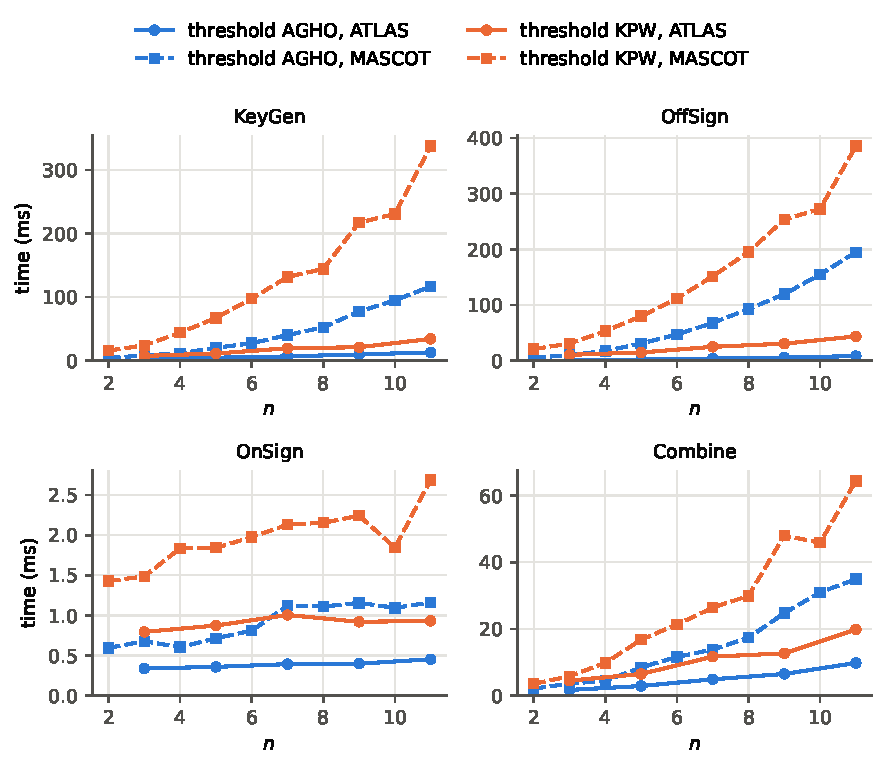
\includegraphics[width=\textwidth]{chapters/03-tsps/tsps-n-times.pdf}
\caption[Threshold SPS schemes: time against $n$]{Time of party $p_1$ against the number of parties $n$, at $\ell = 2$,
median. ATLAS runs at $n = 2t+1$ and MASCOT at $t = n-1$.}
\label{fig:tsps-n-times} \end{figure}

\begin{figure}[htbp] \centering
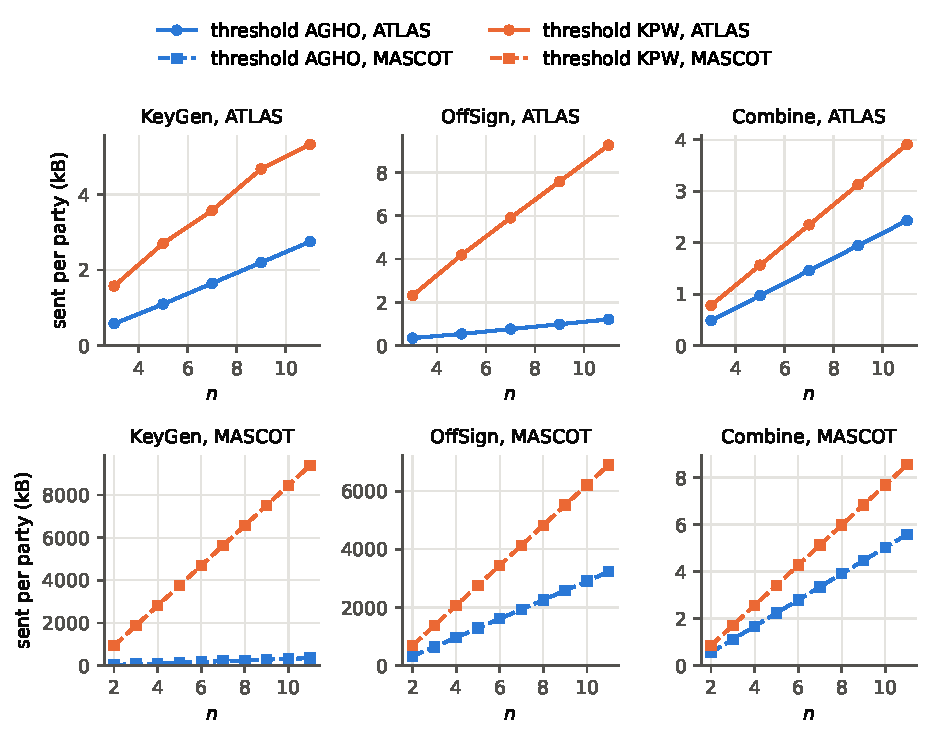
\includegraphics[width=\textwidth]{chapters/03-tsps/tsps-n-comm.pdf}
\caption[Threshold SPS schemes: communication against $n$]{Kilobytes sent by party $p_1$ against the number of parties $n$, at $\ell =
2$, one panel per phase, with ATLAS as solid and MASCOT as dashed lines. MASCOT
sends about a thousand times more, so the ATLAS lines lie close to zero for key
generation and offline signing. $\TSPSonsign$ sends nothing and is not shown.} \label{fig:tsps-n-comm}
\end{figure}

\begin{figure}[htbp] \centering
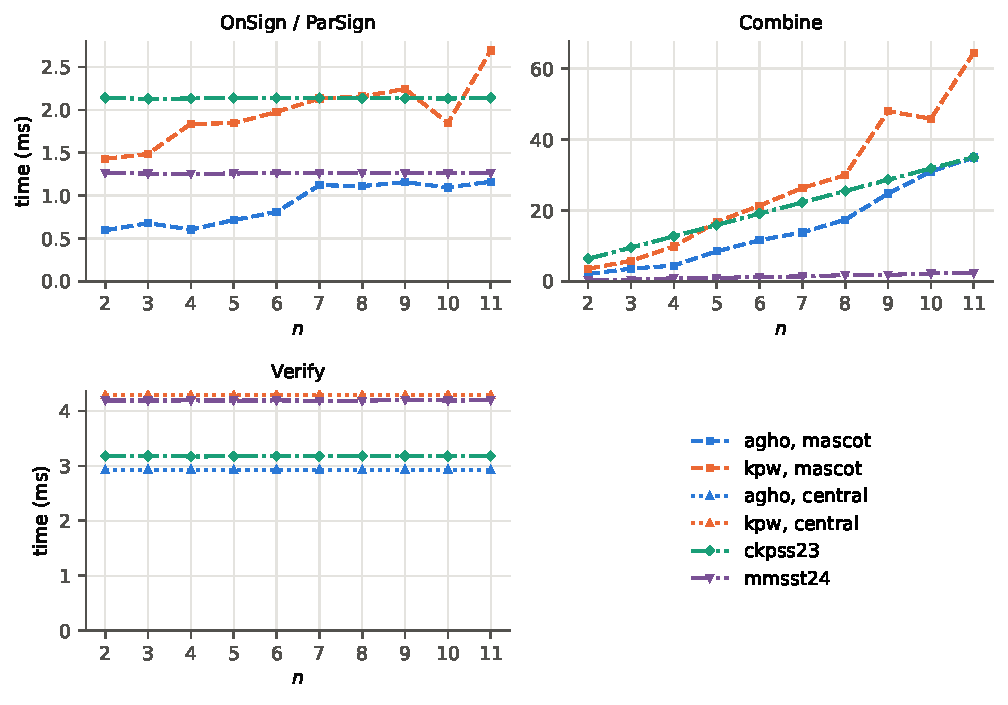
\includegraphics[width=\textwidth]{chapters/03-tsps/tsps-baselines.pdf}
\caption[Threshold SPS schemes against prior schemes]{Our schemes with MASCOT against the prior threshold schemes and the
centralised schemes, against the number of parties $n$, at $\ell = 2$ and $t =
n-1$, median.} \label{fig:tsps-baselines} \end{figure}

